\chapter{Sequence alignment}

\label{kap:sequence_alignment} % id kapitoly pre prikaz ref

In bioinformatics, a sequence alignment is a way of arranging the sequences of DNA, RNA, or protein
to identify regions of similarity that may be a consequence of functional, structural, or
evolutionary relationships between the sequences. \cite{Gollery2005BioinformaticsSA}

As mentioned in the introduction sequences are often extremely hard and can't be aligned by human
and often also by primitive sequence alignment algorithms. Hhuman knowledge is applied in
constructing algorithms to produce high-quality sequence alignments, and occasionally in adjusting
the final results to reflect patterns that are difficult to represent algorithmically (especially in
the case of nucleotide sequences). Computational approaches to sequence alignment generally fall
into two categories: 

\begin{theorem}[Global alignment]
  Global alignment of two sequences $S_{1}$ and $S_{2}$ requires that the alignment $A$ spans the
  entire length of both the sequences $S_{1}$ and $S_{2}$.
\end{theorem}

\begin{theorem}[Local alignment]
  Local alignment of sequences $S_{1}$ and $S_{2}$ allows the optimal alignment $A$ to span only a
  specific region of the sequences. Local alignments are often used to align a shorter sequence to 
  a larger one.
\end{theorem}

\begin{figure}[H]
  \centerline{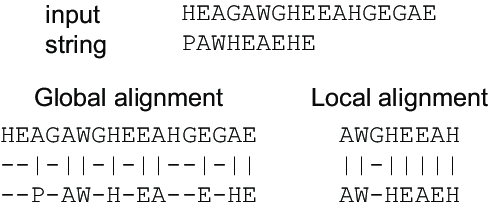
\includegraphics[width=0.8\textwidth]{images/local_global_alignment.png}}
  \caption[Global vs local alignment]{Global vs local alignment}
  \label{obr:local_global_alignment}
\end{figure}

In the following chapter we present the current state of the art algorithms for finding a sequence
alignment. The algorithms have different properties which vary in the running time complexity,
memory, or approximation factor of optimal alignment. Many of the algorithms don't have scientific
guarantees of the optimal solutions and the algorithms rely on the structure of the sequences.

\section{DTW - dynamic time warping}
\label{section:dtw}

Dynamic time warping (DTW) finds similarity between two sequences. It is one of the similarity
methods used in pattern recognition and time series data mining and other fields. Figure 1 shows
example of non-warping and warping between time series. DTW is efficient similarity method for time
series datasets, but it has quadratic time and memory complexity.

\begin{figure}[H]
  \centerline{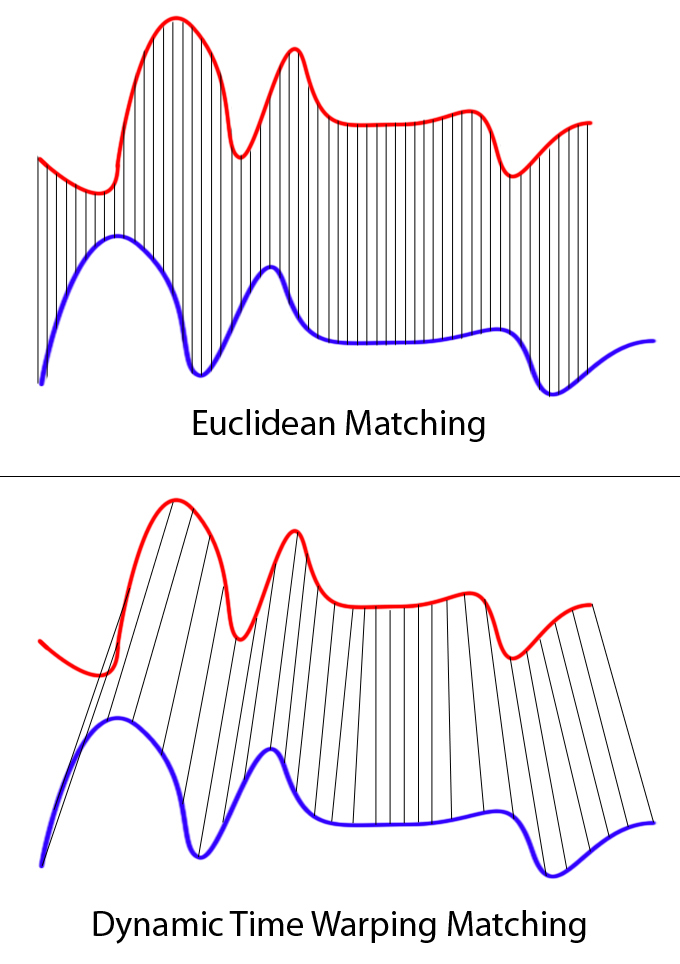
\includegraphics[width=0.4\textwidth]{images/dtw}}
  \caption[DTW]{DTW visualization}
  \label{obr:dtw}
\end{figure}

The algorithm is pretty straightforward. Support we want to calculate alignment $A$ of two sequences
$S = S_1S_2...S_n$ and $T = T_1T_2...T_m$. Note the lengths of the sequences are $n$ and $m$,
respectively. We will build a matrix $M$ of size $n \times m$, where we will be storing the score of
the alignment (we will later show how to reconstruct the alignment itself). The element $M[n][m]$
will be the optimal score of the alignment and we will calculate it recursively using the following
algorithm:

\newcommand\numberthis{\addtocounter{equation}{1}\tag{\theequation}}
\begin{align*}
  M[i][j] = \begin{cases}
    \text{if }  i = 0 & j \\
    \text{else if }  j = 0 & i \\
    \text{else } & C(S_{i}, T_{j}) + min(M[i-1][j], M[i][j-1], M[i-1][j-1]) \numberthis \label{simple_dtw}
  \end{cases}
\end{align*}

where $C(x, y)$ is a cost function which is defined by:

\begin{align*}
  C(x,y) = \begin{cases}
      \text{if }  x = y & 0 \\
      \text{otherwise } & 1
  \end{cases}
\end{align*}

The algorithm checks all possible operations that can happen \textit{insertion, deletion, match or
mismatch}. There is also a variant of the classic DTW algorithm, for which the cost function $C$
returns different values for each type of the operations.

If we want to reconstruct the alignment from the DTW algorithm, we need to create another matrix $P$
with the same dimensions as $M$. Let's call it a path matrix. Initially we set $P[i][j] = (i,j)$ for
all valid $i, j$. We need to modify the algorithm \ref{simple_dtw} to store the best option in the
path matrix $P$. This defines the value of $P[i][j]$:

\begin{align*}
  P[i][j] = \begin{cases}
      \text{if }  i = 0 \text{ or } isMin(M[i][j-1]) & (i, j-1) \\
      \text{else if}  j = 0 \text{ or } isMin(M[i-1][j]) & (i-1, j) \\
      \text{else } & (i-1, j-1)
  \end{cases}
\end{align*}

where the $isMin(x)$ is a function which returns true if the argument is the best choice (leads to
optimal solution).

The alignment is uniquely represented by the operations which led to the optimal alignment
$M[n][m]$. The operations are linked to each other by matrix $P$ and can be obtained recursively
starting at value $P[n][m]$ until $P[i][j] != (i, j)$ (and then reversed).

Note that the running time and memory complexity is $n \times m$, because the whole matrix $M$ needs
to be built. This algorithm is usable only for shorter sequences and ignores the properties of the
sequences. Sequences in this algorithm could be arbitrary strings and we would still get the correct
and optimal alignment. However, comparing arbitrary strings is not the same as comparing sequences
and we might be interested in different scoring methods.

\section{Needleman-Wunsch algorithm}

The Needleman-Wunsch algorithm \cite{NEEDLEMAN1970443}, published in 1970, provides a method of
finding the optimal global alignment of two sequences by maximizing the number of amino acid matches
and minimizing the number of gaps necessary to align the two sequences. When aligning sequences
there are often gaps (i.e. "indels" - insertions and deletions), sometimes large ones. Biologically, a
large gap is more likely to occur as one large deletion as opposed to multiple single deletions.
Hence two small indels should have a worse score than one large one.

The idea of the algorithm is the same as \ref{section:dtw}. The only difference is the
implementation of cost function, which needs to add additional penalty if there is a gap starting.
You can find more about the gap penalty implementation and further improvements in
\cite{Boes2014ImprovingTN}.

\section{FastDTW algorithm}

\section{Efficient DTW Algorithm}
